\documentclass[11pt, letterpaper]{article}

% --- Essential Packages ---
\usepackage[utf8]{inputenc}
\usepackage[margin=1in]{geometry}
\usepackage{amsmath, amssymb, amsthm}  % amsmath for matrices and vectors
\usepackage{graphicx}
\usepackage{hyperref}
\usepackage{listings}                   % for showing code
\usepackage{xcolor}                     % for showing custom colours in code
\usepackage{float}                      % for adding [H] to figures, making them stay in place
\usepackage{booktabs}                   % for table lines

% Custom colours for code files
\definecolor{background}{RGB}{245, 245, 245} % Light grey background

\begin{document}

% --- Custom Single Title Page ---
\begin{titlepage}
    \centering
    \vspace*{0.5in}

    \begin{figure}[H]
        \centering
        \includegraphics[width=0.3\textwidth]{"figures/University_of_Waterloo_seal.png"}
    \end{figure}

    \vspace{1.5cm}

    % Custom Title & Subtitle
    {\Huge \bfseries Lab 2: Controller Design \par}

    \vspace{0.5cm}
    {\Large MTE 484: Digital Control Systems \par}
    \vspace{0.1cm}
    {\Large Instructor Sergio Livera \par}
    \vspace{0.5cm}
    {\large Department of Mechatronics and Mechanical Engineering \par}



    \vfill % Automatically fills vertical space, pushing author/date to the bottom

    % Custom Author Info
    {\Large \textbf{Levi Rogalla} \par}
    {\Large \textbf{Alex Veric} \par}

    \vspace{1.5cm}

    {\large \today \par}

    \vspace*{0.5in}
\end{titlepage}

\clearpage
\thispagestyle{empty}
\begin{center}
    \vspace*{\fill}
    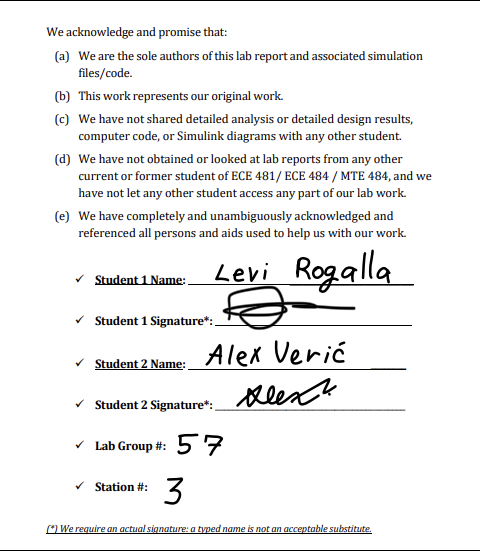
\includegraphics[width=\textwidth,height=0.9\textheight,keepaspectratio]{figures/declaration.png}
    \vspace*{\fill}
\end{center}
\clearpage


\section{Question A}
The controller must be designed in a way that allows the closed loop system to
display the time-domain characteristics required, which are as follows: the
step response steady-state tracking error is zero; he step response 2\%
settling time is no more than 0.25 seconds; the step response overshoot is no
more than 5\%; and the motor voltage does not exceed more than 6V in either
direction. \par
The first requirement is already accounted for due to the nature of our plant.
% Levi: I would say that the open loop system needs to have a model of the reference signal
According to Internal Model Principle, in order for a closed loop system to have
perfect error tracking, the open loop system (which consists of the plant and the controller)
must contain a model of the reference signal in the LaPlace domain. In this situation, the
given reference signal is a step input, which in the LaPlace domain is represented
by $\frac{1}{s}$. The plant being used has already been characterized in the previous
lab, and as can be seen in the following equation, already contains a model of the step
input. Hence, it is not necessary to consider this in the controller design.

\begin{equation}
    P(s) = \frac{K_1}{s(\tau s + 1)}
\end{equation}

Where $K_1 = -1.8906$ and $\tau = 0.018107$.\par

The second two requirements, which regard the 2\% settling time and the overshoot percentage,
must be considered in the design of the controller. These values can be related to the poles
of the closed loop system through the following sets of equations, which will determine the
desired characteristic polynomial; using this information, as well as the previously derived
plant model, the controller can be determined. The following equation shows the relation between the overshoot
percentage and the damping ratio, $\zeta$.

\begin{equation}
    \zeta = - \frac{ln (OS\%)}{\sqrt{\pi^2 + [ln(OS\%)]}}
\end{equation}

The following equation shows the relation between the 2\% settling time, the damping ratio, $\zeta$,
and the natural frequency, $\omega_n$.

\begin{equation}
    \omega_n = \frac{4}{\zeta T_{s_{2\%}}}
\end{equation}

The following equation is the characteristic polynomial of a second order, closed-loop system,
in terms of the damping ratio, $\zeta$, and the natural frequency, $\omega_n$.

\begin{equation}
    \pi(s) = s^2 + 2\zeta \omega_n s + \omega_n
\end{equation}

Substituting $T_{s_{2\%}} = 0.25s$ and $OS\% = 0.05$ into the above equations give the following
values for the damping ratio, $\zeta$ and the natural frequency, $\omega_n$.

\begin{equation}
    \zeta = 0.690, \omega_n = 23.185 [\frac{1}{sec}]
\end{equation}

Substituting these values into the characteristic polynomial gives the following equation:

\begin{equation}
    \pi(s) = s^2 + 31.995s + 537.542
\end{equation}

Using the quadratic formula, as shown below, gives the conjugate pole pair that is required
in the closed-loop system to have the required time-domain characteristics:

\begin{equation}
    \frac{-b \pm \sqrt{b^2 - 4ac}}{2a}
\end{equation}

Where $a = 1$, $b = 31.995$, $c = 537.542$:

\begin{equation}
    s_{1,2} = -15.998 \pm j16.782
\end{equation}

The above poles are the conjugate poles which will determine the behaviour of the closed-loop
system. However, since the lab requires the controller to be at least first-order (and the
derived plant is second order), the characteristic polynomial of the closed-loop system
must be third-order. Thus, another pole is required. In order to maintain the desired behaviour
already determined, this third pole must be non-dominant - this means it must lie on the real
axis and be at least five times further from the imaginary axis than the conjugate pole pair.
The reasoning for this is simple: the real part of a pole is what determines the exponential
behaviour it contributes to the system. If the real value of the pole is significantly larger (and negative)
than the other poles, it will decay much more quickly, resulting in its time-domain behaviour
% Levi: the /par is in the output
% Alex: Addressed
contribution being negligible. \par

Based on the above description, the third and non-dominant pole of the closed-loop system is
$s_3 = -80$. \par

The third-order characteristic polynomial for the system is as follows:

\begin{equation}
    \pi(s) = (s - s_1)(s - s_2)(s - s_3)
\end{equation}

Substituting the three desired poles, $s_1$, $s_2$ and $s_3$:

\begin{equation}
    \pi(s) = (s - (-15.998 + j16.782))(s - (-15.998 - j16.782))(s - (-80))
\end{equation}

Expanding and collecting like terms shows the full third order characteristic polynomial
and its coefficients, which will be used briefly to determine those of the controller.

\begin{equation}
    \pi(s) = s^3 + 111.996s^2 + 3097.252s + 45005.76
\end{equation}

The controller design will be done using the Sylvester matrix method, which will be described
briefly. First, the coefficients of the characteristic polynomial must be gathered:

\begin{equation}
    \alpha_3 = 1, \alpha_2 = 111.996, \alpha_1 = 3097.252, \alpha_0 = 45005.76
\end{equation}

Then, the plant must be made into the following form:

\begin{equation}
    P(s) = \frac{b_2 s^2 + b_1 s - b_0}{s^2 + a_1 s + a_0}
\end{equation}

Taking the plant derived in the previous lab, and transposing it to the above form gives the following:

\begin{equation}
    P(s) = \frac{0 s^2 + 0 s - 104.413}{s^2 + 55.227s + 0}
\end{equation}

And naming the coefficients gives:

\begin{equation}
    b_2 = 0, b_1 = 0, b_0 = -104.413
    a_1 = 55.227, a_0 = 0
\end{equation}

Assuming a proper, first-order controller of the following form:

\begin{equation}
    \label{eq:controller_model}
    C(s) = \frac{g_1 s + g_0}{f_1 s + f_0}
\end{equation}

Now, the Sylvester matrix method will be described. It states that a matrix
made up of the coefficients of the plant, called the Sylvester matrix, multiplied
by an array made up of the coefficients of the controller is equal to an array
made up by the coefficients of the resulting characteric polynomial. The following
equation displays this:

\begin{equation}
    \begin{bmatrix}
        1   & 0   & b_2 & 0   \\
        a_1 & 1   & b_1 & b_2 \\
        a_0 & a_1 & b_0 & b_1 \\
        0   & a_0 & 0   & b_0
    \end{bmatrix}
    \begin{bmatrix}
        f_1 \\
        f_0 \\
        g_1 \\
        g_0
    \end{bmatrix}
    =
    \begin{bmatrix}
        \alpha_3 \\
        \alpha_2 \\
        \alpha_1 \\
        \alpha_0
    \end{bmatrix}
\end{equation}

Substituting all the gathered coefficients from the desired characteristic polynomial and the
plant gives:

\begin{equation}
    \begin{bmatrix}
        1      & 0      & 0        & 0        \\
        55.227 & 1      & 0        & 0        \\
        0      & 55.227 & -104.413 & 0        \\
        0      & 0      & 0        & -104.413
    \end{bmatrix}
    \begin{bmatrix}
        f_1 \\
        f_0 \\
        g_1 \\
        g_0
    \end{bmatrix}
    =
    \begin{bmatrix}
        1        \\
        111.996  \\
        3097.252 \\
        43005.760
    \end{bmatrix}
\end{equation}

Using simple system of equation rules allows for the calculation of each controller coefficient, as
follows:

\begin{equation}
    f_1 = 1, f_0 = 56.769, g_1 = 0.363, g_0 = -411.881
\end{equation}

Substituting these values into the controller model from equation \ref{eq:controller_model} gives the following:

\begin{equation}
    C(s) = \frac{0.363s - 411.881}{s + 56.769}
\end{equation}

The above controller model was placed into the closed-loop simulation model in MatLab, with the
previously derived plant. The reference signal was set to a step function which alternates between
$-0.7 rad$ and $0.7 rad$, with a duty cycle of 50\% and a period of 2 seconds, as instructed. Below is
the model, followed by the time-domain response.

\begin{figure}[H]
    \centering
    \includegraphics[width=0.7\textwidth]{"figures/closed-loop-model-controller.png"}
    \caption{Model of closed-loop system.}
\end{figure}

\begin{figure}[H]
    \centering
    \label{fig:time-domain-response-pre-tweak}
    \includegraphics[width=0.7\textwidth]{"figures/time-domain-response-pre-tweak.png"}
    \caption{Time-domain response of closed-loop system to reference signal.}
\end{figure}

From figure \ref{fig:time-domain-response-pre-tweak}, it is clear that the steady state error
is equal to zero. In order to determine if the controller meets the other two requirements,
the peak value and the settling time of the time-domain response signal must be measured.

\begin{figure}[H]
    \centering
    \label{fig:time-domain-meas-settling-time-pre-tweak}
    \includegraphics[width=0.7\textwidth]{"figures/time-domain-meas-settling-time-pre-tweak.png"}
    \caption{Measurement of 2\% settling time}
\end{figure}

\begin{figure}[H]
    \centering
    \label{fig:time-domain-meas-overshoot-pre-tweak}
    \includegraphics[width=0.7\textwidth]{"figures/time-domain-meas-overshoot-pre-tweak.png"}
    \caption{Measurement of overshoot percentage}
\end{figure}

The 2\% settling time is the amount of time after the step response that is required
for the system output to reach 2\% of the reference signal. Since the reference signal goes
from $-0.7$ to $0.7$, the total value of the step function is $1.4$. Therefore, the 2\% settling
time occurs when the signal reaches $102\%$ of $1.4$, which is $1.428$. The measurement in figure
\ref{fig:time-domain-meas-settling-time-pre-tweak} shows that this occurs $0.275$s after the
unit step, which is slower than the required $0.25$s. \par
The overshoot percentage, which is required to be no more than 5\%, is measured in figure
\ref{fig:time-domain-meas-overshoot-pre-tweak}. The peak difference is measured to be $1.464$;
$105\%$ of the unit step value would be $1.47$, and so the overshoot percentage of this controller
is within the acceptable range. \par

Since the 2\% settling time is dependent on the natural frequency, $\omega_n$, this would need to
be modified in order to prevent the settling time from going above its limit. However, this would
be time consuming, as it would require redoing nearly the entire process as described above.
\verb|systune|, a tool in MatLab, is a much more efficient way of tuning the
existing controller to fit within the required settling time. The newly tuned controller has
the following values, and its response to a step input can be seen in figure
\ref{fig:step-response-post-tune}.

\begin{equation}
    \label{eq:tuned_controller}
    C(s) = \frac{-2.452 s - 135.4}{s + 24.95}
\end{equation}

\begin{figure}[H]
    \centering
    \label{fig:step-response-post-tune}
    \includegraphics[width=0.3\textwidth]{"figures/step-response-post-tune.png"}
    \caption{Tuned controller performance to step input.}
\end{figure}

The tuned controller has a $2\%$ settling time of $0.2252s$ and an overshoot percentage of exactly
$2.00\%$, both of which fit the required time-domain performance.
The new controller is also shown to have a voltage within $\pm 6V$, as can be
seen by the signal output by C(s) in figure \ref{fig:cont-controller-voltage}.

\begin{figure}[H]
    \centering
    \label{fig:cont-controller-voltage}
    \includegraphics[width=0.7\textwidth]{"figures/cont-controller-voltage.png"}
    \caption{Motor voltage shown to be within $\pm 6V$ when using the tuned controller.}
\end{figure}

\section{Question B}

The discretization of a controller is necessary to allow a microcontroller, such as the Arduino Mega,
to run the controller digitally. Software controllers cannot run in continuous time, and so have
to sample the continuous time values, therefore making the system discrete. While a continuous controller
can use derivatives to transform between LaPlace and time domains, discrete systems are non-continuous
and therefore can not utilize derivatives. This results in discretization being necessary, and this
can be done using one of two methods: bilinear transformation or step-invariant transformation.
Bilinear transformation guarantees the stability of an already stable continuous controller, and
is better at maintaining the time-domain behaviour of a continuous controller, while
step-invariant transformation does not guarantee stability, but better maintains frequency domain
responses. Since time-domain characteristics are those which are required, and stability is
paramount in this system, bilinear transformation will be used to discretize the continuous
controller. \par

Bilinear transformation involves replacing the Laplace domain variable $s$ with the discrete domain
variable $z$, using the following equation:

\begin{equation}
    \label{eq:bilinear-transform}
    s = \frac{2}{T}\frac{z-1}{z+1}
\end{equation}

Where $T$ is the sampling period, which has been chosen to be 0.0005, making the sampling frequency equal
to $2kHz$. Analyzing the time-domain step response, there are a few periods in which fast response is
important, such as the peak time
and the settling time, which are required characteristics that must be maintained during discretization.
At these points, the controller must react quickly to limit the overshoot around the peak time
and to reduce oscillations around the 2\% settling time. Since the time constant which governs these values
is 0.0625, the sampling time period was chosen to be roughly one hundred times smaller to allow the controller to
react appropriately. \par
(Note: 200 Hz was initially used for the sampling frequency, but it was experimentally determined that this was too slow of
a response to obtain the desired time-domain characteristics; for this reason, the frequency was increased by a factor of ten.)

Substituting $s$ using equation \ref{eq:bilinear-transform} into the equation
\ref{eq:controller_model} for the continuous controller gives a new, discrete controller
formula that should replicate its time-domain behaviour:

\begin{equation}
    C[z] = \frac{(2g_1+Tg_0)z + (Tg_0 - 2g_1)}{(2f_1+Tf_0)z + (Tf_0 - 2f_1)}
\end{equation}

Substituting the new coefficients of the tuned controller, as seen in equation
\ref{eq:tuned_controller}, as well as the chosen sampling period, $T$, gives the following:

\begin{equation}
    \label{eq:discrete-z-domain-controller}
    C[z] = \frac{-4.9717z+4.8363}{2.012475z-1.987525}
\end{equation}

The discrete controller was then input into MatLab, where it was compared with the continuous
controller step response.

\begin{figure}[H]
    \centering
    \label{fig:discrete-controller-model}
    \includegraphics[width=0.7\textwidth]{"figures/discrete-controller-model.png"}
    \caption{Discrete controller model in MatLab}
\end{figure}

\begin{figure}[H]
    \centering
    \label{fig:discrete-step-response-matlab}
    \includegraphics[width=0.7\textwidth]{"figures/discrete-step-response-matlab.png"}
    \caption{Discrete and continuous models step response compared. As can be seen, there is little to no visible difference between the time-domain characteristics of the two models.}
\end{figure}

\begin{figure}[H]
    \centering
    \label{fig:discrete-controller-voltage-matlab}
    \includegraphics[width=0.7\textwidth]{"figures/discrete-controller-voltage-matlab.png"}
    \caption{Motor voltage when using the discrete controller; it does not encroach $\pm 6V$}
\end{figure}

\section{Question C}
Now that the controller has been discretized, it can now be used to run the control
system on the Arduino, which works digitally and in fixed sample intervals. However,
there is one last step before the Arduino can use the controller: it must be
transformed from the Z-domain into the sampling domain, which, unlike its counterpart,
the time-domain, computes in fixed time intervals rather than continuous time. In order
to do this, the controller must first be represented in terms of the signals which act
as its input and output, as seen below:

\begin{equation}
    C[z] = \frac{U[z]}{E[z]} = \frac{-4.9717z+4.8363}{2.012475z-1.987525}
\end{equation}

Where U[z] is the discrete output of the controller, and E[z] is the discrete input.
This equation must be rearranged as follows, to obtain a value for the output,
based on the input:


\begin{equation}
    U[z] = \frac{-4.9717z+4.8363}{2.012475z-1.987525} E[k]
\end{equation}

Applying the inverse Z-transform:

\begin{equation}
    u[k] = 0.987602u[k-1] - 2.470441e[k] + 2.403160e[k-1].
\end{equation}

Where $k$ is an arbitrary sample, similar to how $t$ is an arbitrary continuous unit of time,
in the time-domain. The above equation was implemented in the Arduino code, along with
its appropriate sampling time of $0.0005s$. The entire system was then tested with the
a square wave input signal at $50\%$ duty cycle and with a period of $2s$. The system
time response is shown below in figure \ref{fig:real-controller-time-response}.

\begin{figure}[H]
    \centering
    \label{fig:real-controller-time-response}
    \includegraphics[width=0.7\textwidth]{"figures/real-controller-time-response.png"}
    \caption{Step response of the motor}
\end{figure}

In order to ensure the time-domain characteristics required for this system are reached, figure
\ref{fig:real-controller-time-response} must be further inspected. The $2\%$ settling time
is reached almost exactly $0.25s$ after the step input is triggered. Additionally, the peak
of the motor position is $0.72087 rad$, which is roughly $2\%$ of the unit step value; this meets
the required maximum overshoot percentage of $5\%$. See below the exact values of the first recorded
time-domain response from figure \ref{fig:real-controller-time-response}:

\[
    \begin{aligned}
        \text{2\% range}                & = (0.672, 0.728),       \\
        T_{\text{signal}}               & = 19.7017315\,\text{s}, \\
        T_{s,\,2\%}                     & = 19.951723\,\text{s},  \\
        T_{s,\,2\%} - T_{\text{signal}} & = 0.2499915\,\text{s}.
    \end{aligned}
\]

Using the following equations to obtain $OS\%$:

\begin{equation}
    OS\% = \frac{u(t)_{max} - r(t)_{max}}{|r(t)|} \times 100\%
\end{equation}

The following OS\% can be obtained:

\begin{equation}
    OS\% = 1.43928\%
\end{equation}

The figure below shows the motor voltage as well, which never exceeds $\pm 6V$:

\begin{figure}[H]
    \centering
    \includegraphics[width=0.7\textwidth]{"figures/real-controller-motor-voltage.png"}
    \caption{Step response and voltage of motor.}
\end{figure}

There are several differences between the performance of the simulated system
and the real system when using the discretized controller. The $2\%$ settling time
of the real system is slightly longer than the simulated one, which can likely be attributed
to the time delay introduced by the controller running on real hardware rather than inside
a simulation. This presents itself in the form of a very slight delay between the unit step and the
beginning of the motor movement, as can be seen in figure \ref{fig:real-controller-zoomed}, which doesn't exist
in the simulated system, in figure \ref{fig:step-response-post-tune}

\begin{figure}[H]
    \centering
    \label{fig:real-controller-zoomed}
    \includegraphics[width=0.7\textwidth]{"figures/real-controller-zoomed.png"}
    \caption{Zoomed in chart of the motor step response.}
\end{figure}

The experimental overshoot percentage is smaller than the simulated system. This was expected,
as the forces introduced in a real system, such as internal friction or air resistance, increase the
damping ratio of the system, resulting a smaller overshoot. The motor voltage of the system was seen to
be higher than that of the simulated system, which was, once again, expected behaviour. The constant voltage
added to the motor voltage by the Arduino code was one culprit of this higher motor voltage, as was the
controller having to add more voltage as a result of the aforementioned internal friction and air resistance
which do not exist in the simulated system.

\section{Question D}

The stiction values from Lab 1 were found to no longer hold up when the system had increased weight due to
the beam now being attached. The new stiction values were found in the same way as before: a program
was used to increase the motor voltage from zero in very small increments until the motor began to move -
this was done in both directions. The values were changed for both directions, since the beam being attached
to the motor gear changes the voltage required for both directions. In the clockwise direction, the beam
pushes in the direction of the motor movement, which means the controller does not need to accout for as much stiction as before. In the counter-clockwise
direction, the beam pushes in the opposite direction of the motor movement, meaning the controller must use a higher
voltage than before to overcome the stiction. While running this program, it was imperative that the ball was on the beam,
as this was another factor that would contribute weight to the system, and so the stiction values needed
to account for this. \par
The program implemented to determine the stiction values worked as followed. The inner-loop controller
was used to set the motor angle to zero. Once there, the voltage required to do so was recorded and used
as the basepoint. From here, the voltage would increase in very small increments until the motor
was recorded to have moved in the desired direction. At this point, the program would stop and
output the difference in voltage from the basepoint to the amount required to move the motor. This
was done for both sides. \par

As can be seen in figure \ref{fig:stiction-chart}, unless the motor voltage is set to zero, the output of the controller
always causes the motor to move; this is the succesful result of finding the correct stiction values
and accomodating for them in code.


The values for stiction were found to be $-0.5763 V$ in the counter-clockwise direction, and $-0.1034 V$ in
the clockwise position.

\begin{figure}[H]
    \centering
    \label{fig:stiction-chart}
\end{figure}

The emergency stop function, which stops the motor function at a certain motor position ($\pm 0.8 rad$)
to stop potential damage to the system, was also implemented in the code, in the following way.
The motor angle is checked continuously by the control interrupt. If its magnitude exceeds
$0.8\ \mathrm{rad}$, the motor voltage is set to zero, the controller is disabled, and the
system switches to the emergency stop state. This prevents the controller from driving the
motor further and helps prevent damage to the system.

As can be seen in figure \ref{fig:estop-chart}, the emergency stop works as intended.

\begin{figure}[H]
    \centering
    \label{fig:estop-chart}
\end{figure}

\section{Question E}

Now that the inner control loop, which transforms the desired motor angle values into accurate
motor movement, is almost complete, it is time to start working towards the outer control loop,
which must determine the motor angle required in order to move the ball towards a specific
position on the beam. A required step in this process is to have an effective method
of determining the position of the ball on the beam; this will be used in the outer
loop's error measurements. The beam has a built in sensor, whose output represents the current
position of the ball; however, the sensor must be characterized in order to determine
how the sensor value corresponds to the position of the ball on the beam in meters. \par

This can be done using the following formula as a conversion between sensor output and
ball position:

\begin{equation}
    \label{eq:beam-sensor-linearization}
    p_{radians} = m \times p_{sensor} + b
\end{equation}

Where the $m$ and $b$ values must be determined through a system of equations, using
experimental values of $p_{meters}$ and $p_{sensor}$ to do so. \par

The position of the ball on the beam was manually changed to two different points:
one at each the furthermost left and right side of the beam. These two points are
sufficient to determine a linear relationship. Using the measurement convention
given in the lab manual, it must be noted that the ball will never reach $0m$ or $L m$,
where $L$ is the length of the beam; this is due to the small stoppers that rest at each
end of the beam to ensure the ball doesn't fall off.  At each point,
the distance from the beam origin was measured, and the value printed into the serial monitor
was also noted, providing values of $p_{meters}$ in meters and $p_{sensor}$ in ADC counts. It
should also be mentioned that each ADC "value" recorded in this report is actually the
average of multiple ADC values at that specific ball position, effectively reducing the effect of
ADC and sensor noise.\par
The following values were noted:

\[
    \begin{aligned}
        p_{meters_{0}} = 0.030m, p_{sensor_{0}} = 2322.44
        p_{meters_{1}} = 0.389m, p_{sensor_{1}} = 35333.44
    \end{aligned}
\]

The following system of equations was then made from the above values:

\begin{equation}
    \begin{bmatrix}
        0.030 \\
        0.389
    \end{bmatrix}
    =
    \begin{bmatrix}
        2322.44  & 1 \\
        35333.44 & 1
    \end{bmatrix}
    \begin{bmatrix}
        m \\
        b
    \end{bmatrix}
\end{equation}

The above system of equations was solved for $m$ and $b$ resulting in the following values:

\begin{equation}
    \label{eq:beam-sensor-values}
    m = 1.0875 \times 10^{-5}, b = 4.7431 \times 10^{-3}
\end{equation}

After implemented equation \ref{eq:beam-sensor-linearization} into the Arduino code,
using the values provided from
equation \ref{eq:beam-sensor-values}, the ball position could now be determined using
the beam sensor output.

\section{Question F}

Now that the ball position can reliably be determined, it is now necessary to determine
the relation between the input and the output of the outer-loop controller, which will be
the ball location and the motor gear angle, respectively. This transfer function has two parts:
the first is the transfer function between the motor gear angle and the beam angle. This has
already been determined in the lab manual to be the equation
\ref{eq:motor-angle-beam-angle-transfer-function}.

\begin{equation}
    \label{eq:motor-angle-beam-angle-transfer-function}
    \frac{\Phi (s)}{\Theta (s)} = 0.0609
\end{equation}

Where $\Phi(s)$ represents the beam angle, and $\Theta(s)$ represents the motor angle. The second
part is the relation between the beam angle and the ball position, which takes the form
of equation \ref{eq:beam-angle-ball-position-transfer-function}.

\begin{equation}
    \label{eq:beam-angle-ball-position-transfer-function}
    \frac{Y(s)}{\Phi (s)} = \frac{K_3}{s^2}
\end{equation}

Where $Y(s)$ represents the position of the ball on the beam.
Rearranging equation \ref{eq:beam-angle-ball-position-transfer-function} and applying the
inverse Laplace transform provides the following equation:

\begin{equation}
    \label{eq:time-domain-acceleration-relation}
    \ddot{y}(t) = K_3 \phi (t)
\end{equation}

Which shows that $\ddot{y}(t)$, which represents the second derivative of position, also known
as acceleration, is dependent on the beam angle. The knowledge of the basic kinematics
equation which defines acceleration is shown below:

\begin{equation}
    \label{eq:kinematics-acceleration}
    y(t) = y_0 + \dot{y}_0 (t-t_0) + \frac{1}{2} \ddot{y} (t - t_0)^2
\end{equation}

Substituting equation \ref{eq:time-domain-acceleration-relation} into equation \ref{eq:kinematics-acceleration}
heeds the following equation:

\begin{equation}
    y(t) = y_0 + \dot{y}_0 (t - t_0) + \frac{1}{2} K_3 \phi (t - t_0)^2
\end{equation}

Isolating for $K_3$ gives the following:

\begin{equation}
    \label{eq:k3-isolated}
    K_3 = 2 \frac{y - y_0 - \dot{y}_0 (t-t_0)}{\phi (t-t_0)^2}
\end{equation}

Where $y$ is the current position of the ball, $y_0$ is the initial position of the ball,
$\dot{y}_0$ is the initial speed of the ball, $\phi$ is the beam angle for the given
experiment, $t_0$ is the initial time the ball is placed
and $t$ is the current time at which $y$ is being measured. \par

The experiments were then performed to determine $K_3$. At a given beam angle and initial time, the ball would
be placed at a given initial position, at the initial speed of zero. At any arbitrary point of
time in the drop, the position and its time can be inputted into the equation, allowing for the
value of $K_3$ to be solved. This experiment was performed six times, at three different positive
beam angles and three different negative angles, to ensure that the value of $K_3$ was consistent
across all different beam angles. The following beam angles were chosen, as they were determined
to be representative of those used while controlling the ball position. The inner-loop controller
was used to fix the beam at a specific angle, allowing for the experiment to take place.

\[
    \begin{aligned}
        \phi_0 & = 0.2 rad,  &
        \phi_1 & = -0.2 rad, &
        \phi_2 & = 0.3 rad,    \\
        \phi_3 & = -0.3 rad, &
        \phi_4 & = 0.4 rad,  &
        \phi_5 & = -0.4 rad
    \end{aligned}
\]

The figure below shows the entire experiment process,
including all six different beam angles.

\begin{figure}[H]
    \centering
    \label{fig:acceleration-test}
    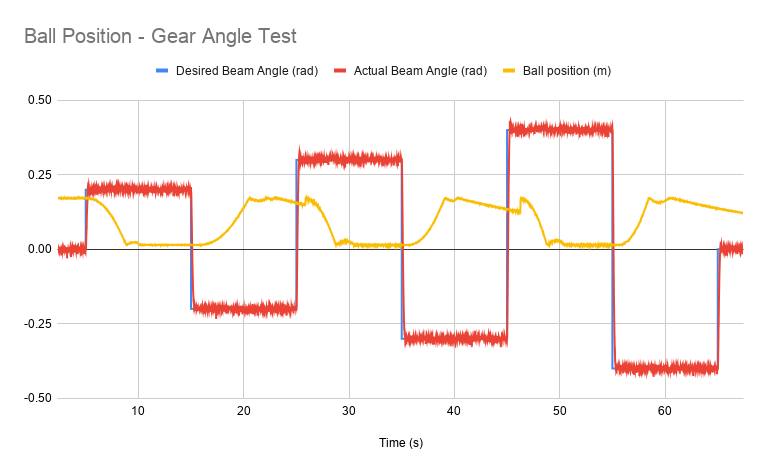
\includegraphics[width=0.7\textwidth]{figures/acceleration-test.png}
    \caption{Experimental determination of $K_3$}
\end{figure}

From the above data, the values for $y$, $y_0$, $\dot{y}_0$, $t_0$, $t$ and $\phi$ can be recorded for
each experiment, as is shown in the table below:

\begin{table}[htbp]
    \centering
    \small
    \setlength{\tabcolsep}{3pt}
    \caption{Ball position - Gear Angle test}
    \label{tab:acceleration-test}
    \begin{tabular}{cccccc}
        \toprule
        \shortstack{\textbf{Beam angle}                            \\$\boldsymbol{\phi}$ \textbf{[rad]}} &
        \shortstack{\textbf{Current ball}                          \\\textbf{position} $y$ \textbf{[m]}} &
        \shortstack{\textbf{Initial ball}                          \\\textbf{position} $y_0$ \textbf{[m]}} &
        \shortstack{\textbf{Initial ball speed}                    \\$\dot{y}_0$ \textbf{[m/s]}} &
        \shortstack{\textbf{Current time}                          \\$t$ \textbf{[s]}} &
        \shortstack{\textbf{Initial time}                          \\$t_0$ \textbf{[s]}} \\
        \midrule
        0.2  & 0.11829066 & 0.17151371 & 0 & 7.321955  & 5.187743  \\
        -0.2 & 0.0964533  & 0.01474824 & 0 & 19.195892 & 15.310882 \\
        0.3  & 0.05731362 & 0.16755515 & 0 & 28.310871 & 26.289441 \\
        -0.3 & 0.14961113 & 0.01784766 & 0 & 38.823754 & 36.122445 \\
        0.4  & 0.06996144 & 0.15256917 & 0 & 48.298498 & 47.134454 \\
        -0.4 & 0.14098713 & 0.01495486 & 0 & 58.162953 & 55.559953 \\

        \bottomrule
    \end{tabular}
\end{table}

Substituting the above values into equation \ref{eq:k3-isolated} provides the following values for
$K_3$:

\begin{table}[htbp]
    \centering
    \caption{Experimental values of $K_3$}
    \label{tab:k3-results}
    \begin{tabular}{cc}
        \toprule
        \textbf{Beam angle $\phi$ [rad]} & \textbf{$K_3$ constant} \\
        \midrule
        0.2                              & -0.11684890             \\
        -0.2                             & -0.05413332             \\
        0.3                              & -0.17986082             \\
        -0.3                             & -0.12038025             \\
        0.4                              & -0.30482592             \\
        -0.4                             & -0.09300439             \\
        \bottomrule
    \end{tabular}
\end{table}

Averaging out the values gives a final result for $K_3$:

\[
    K_{3_{avg}} = -0.14484227
\]

\section{Question G}
\begin{figure}

    \centering
    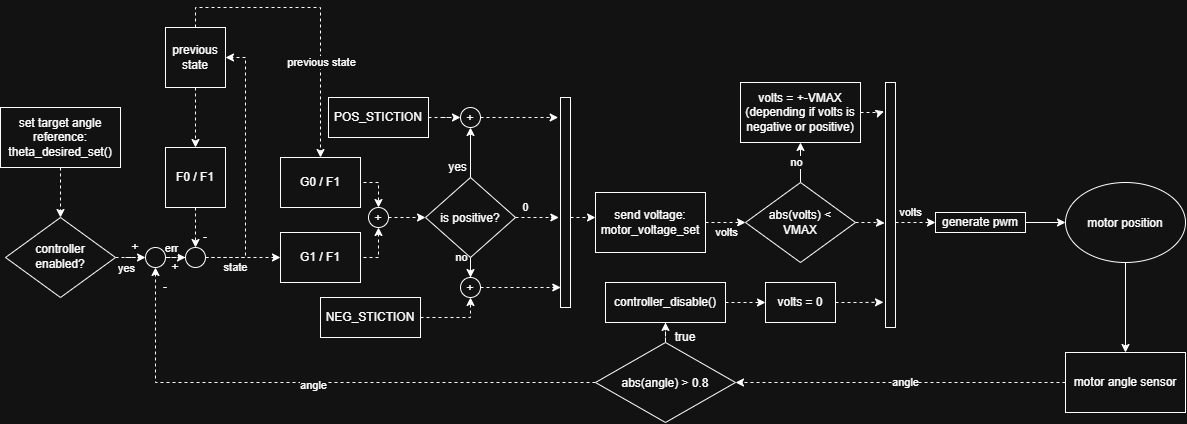
\includegraphics[width=1.2\textwidth, angle=270]{figures/control_system_block_diagram.png}
    \caption{Block Diagram}
\end{figure}

\clearpage
\section*{References}
\begin{enumerate}
    \item S. Livera, \emph{MTE 484: Digital Control Systems --- Lab 2}, Fall 2026.
\end{enumerate}

\section{Appendices}

\subsection{Appendix A: Lab 1 Motor Parameters}

The following table summarizes the motor and gear-angle calibration values
determined in Lab 1. The $K_1$ and $\tau$ values for $K_p=-28$ are used in
the motor model in this report.

\begin{table}[htbp]
    \centering
    \small
    \caption{Motor and gear-angle calibration values from Lab 1}
    \label{tab:lab1-parameters}
    \begin{tabular}{lll}
        \toprule
        \textbf{Parameter}             & \textbf{Value}    & \textbf{Units / description}         \\
        \midrule
        $K_1$ ($K_p=-25$)              & $-1.6413$         & $\mathrm{rad/(V\,s)}$                \\
        $\tau$ ($K_p=-25$)             & $0.019909$        & $\mathrm{s}$                         \\
        $K_1$ ($K_p=-28$)              & $-1.8906$         & $\mathrm{rad/(V\,s)}$; used in Lab 2 \\
        $\tau$ ($K_p=-28$)             & $0.018107$        & $\mathrm{s}$; used in Lab 2          \\
        $K_1$ ($K_p=-30$)              & $-1.8103$         & $\mathrm{rad/(V\,s)}$                \\
        $\tau$ ($K_p=-30$)             & $0.018144$        & $\mathrm{s}$                         \\
        Positive stiction offset $v_+$ & $+0.120$          & $\mathrm{V}$                         \\
        Negative stiction offset $v_-$ & $-0.101$          & $\mathrm{V}$                         \\
        Gear-angle scale $m$           & $-0.000359453251$ & $\mathrm{rad/count}$                 \\
        Gear-angle offset $b$          & $1.75789534$      & $\mathrm{rad}$                       \\
        \bottomrule
    \end{tabular}
\end{table}

The gear-angle conversion is
\[
    \theta = -0.000359453251\,p_{\mathrm{sensor}} + 1.75789534,
\]
where $p_{\mathrm{sensor}}$ is the measured sensor value in ADC counts.

\subsection{Appendix B: Code}

\lstinputlisting[
    language=C++,
    caption={main.ino},
    backgroundcolor=\color{background},
    breaklines=true,
    frame=single
]{../../main/main.ino}

\lstinputlisting[
    language=C++,
    caption={motor.h},
    backgroundcolor=\color{background},
    breaklines=true,
    frame=single
]{../../main/src/motor.h}

\lstinputlisting[
    language=C++,
    caption={motor.cpp},
    backgroundcolor=\color{background},
    breaklines=true,
    frame=single
]{../../main/src/motor.cpp}

\lstinputlisting[
    language=C++,
    caption={position.h},
    backgroundcolor=\color{background},
    breaklines=true,
    frame=single
]{../../main/src/position.h}

\lstinputlisting[
    language=C++,
    caption={position.cpp},
    backgroundcolor=\color{background},
    breaklines=true,
    frame=single
]{../../main/src/position.cpp}

\lstinputlisting[
    language=C++,
    caption={transfer.h},
    backgroundcolor=\color{background},
    breaklines=true,
    frame=single
]{../../main/src/transfer.h}

\lstinputlisting[
    language=C++,
    caption={transfer.cpp},
    backgroundcolor=\color{background},
    breaklines=true,
    frame=single
]{../../main/src/transfer.cpp}

\lstinputlisting[
    language=C++,
    caption={geeWhiz.h},
    backgroundcolor=\color{background},
    breaklines=true,
    frame=single
]{../../main/src/geeWhiz/geeWhiz.h}

\lstinputlisting[
    language=C++,
    caption={geeWhiz.cpp},
    backgroundcolor=\color{background},
    breaklines=true,
    frame=single
]{../../main/src/geeWhiz/geeWhiz.cpp}




\end{document}